\subsection{Beschreibung HMI - Datenbank}
\label{kap:ClientGraphProgrammDatenbank}
W�hrend des Aufzeichnens von Sensorwerten erfolgt das Abspeichern in eine Datenbank. Diese beinhaltet die Daten f�r jeden Sensor einzeln mit den Beschleunigungswerten in x, y und z, sowie einen Zeitstempel. Die Datenbank kann durch das Bet�tigen des Buttons \textit{Show Database}, in der Hauptansicht des Programms, angezeigt werden (s. Abbildung \ref{fig:clientgraphdatabase}).\\
Bei einer ernueten Messwertaufnahme wird der Datenbankinhalt gel�scht.

\begin{figure}[H]
\centering
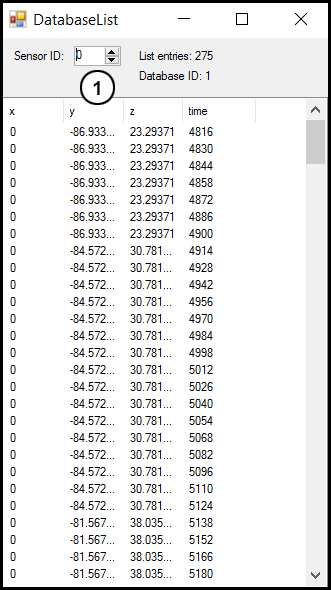
\includegraphics[width=0.5\linewidth]{03_Grafiken/Messsystem/ClientGraphDatabase}
\caption[Datenbank mit Sensorwerten]{Datenbank mit Sensorwerten}
\label{fig:clientgraphdatabase}
\end{figure}
